\setcounter{secnumdepth}{-1}

\chapter{Introduction}

This report aims to complete the code that simulates a DVB-C transmission chain in matlab. It provides additionnal information from the theoretical part of the project. \\
The first part aims to simulate each block of the transmission chain and to link them together such that the received signal is the same as the transmitted signal (in a noiseless case). \\

\Large{Second part to be explained later}
\normalsize

\vspace{2cm}

\begin{figure}[H]
    \centering
    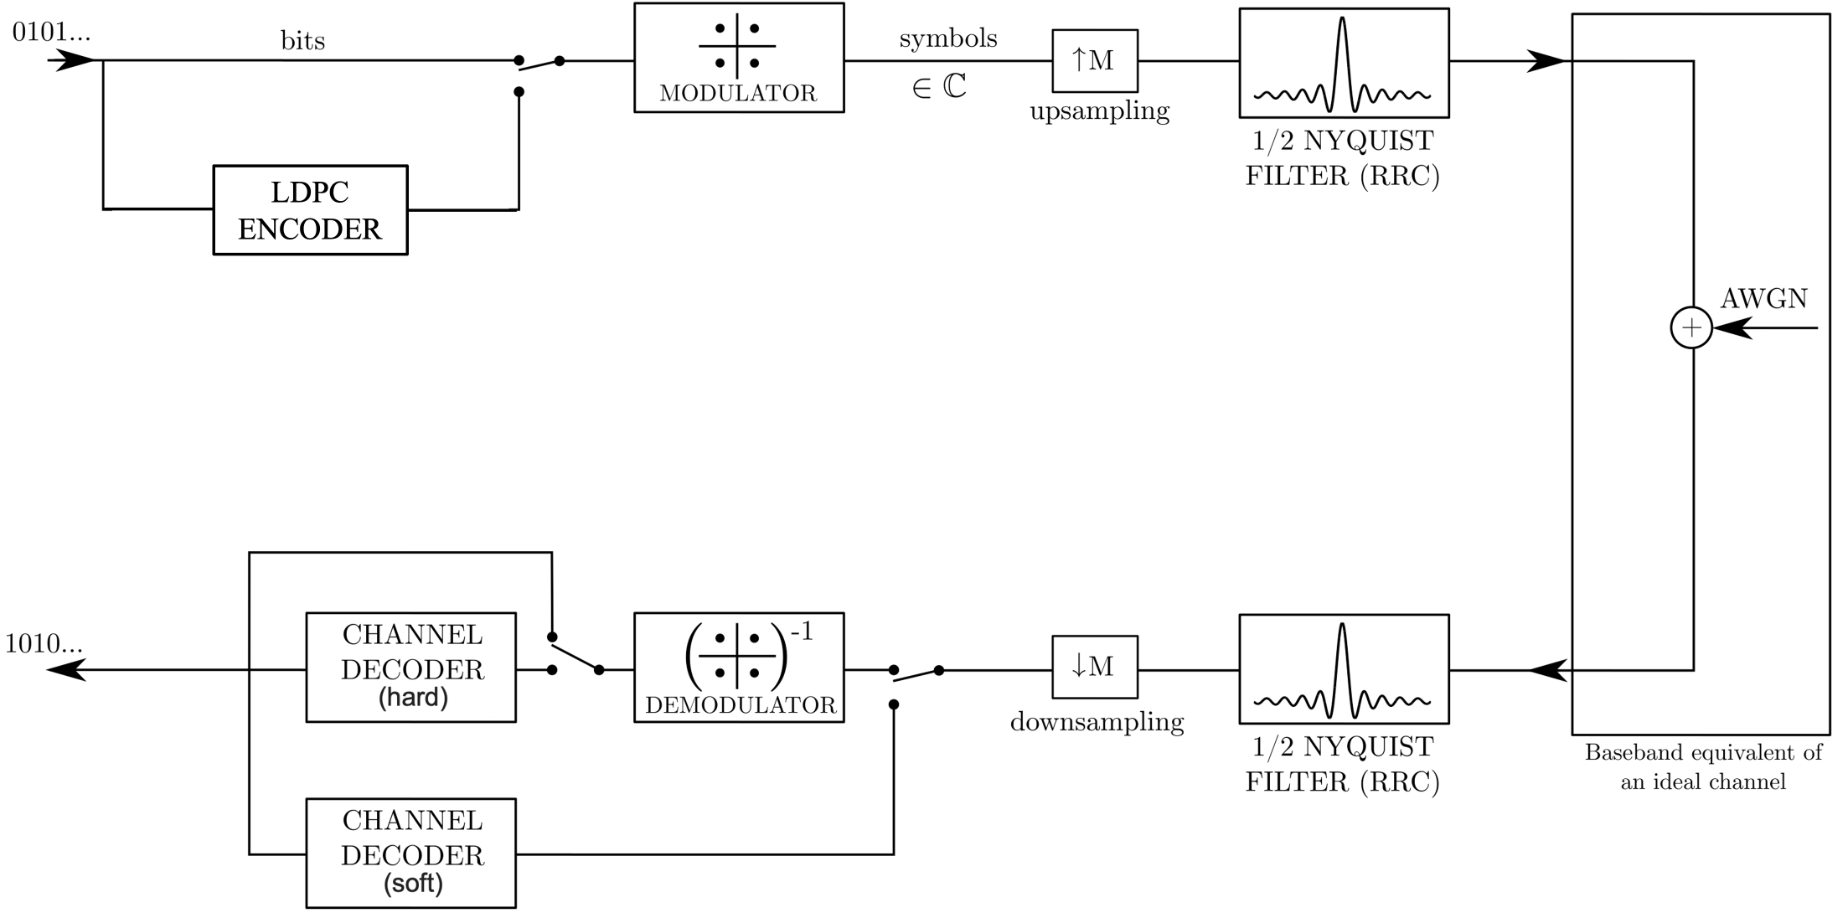
\includegraphics[width=0.9\linewidth]{blockDiagram.png}
    \caption{DVB-C transmission chain}
    \label{fig:blockDiagram}
\end{figure}
